\subsection{ Osservatori uniformemente accelerati}
Si considera una particella $P_0$, uniformemente accelerata rispetto al sistema istantaneamente inerziale  $\mathcal{I}$.
Il sistema $\mathcal{I}$ va inteso come un insieme di sistemi di riferimento inerziali, tra i quali, per ogni tempo, si considera quello rispetto a cui la particella $P_0$ \`e istantaneamente ferma.
\subsubsection{Particella accelerata}
Si considera una generica particella $P$, con velocit\`a $u$ e accelerazione $a$ nel sistema $\mathcal{I}$.
Il boost a velocit\`a inversa dal sistema in movimento $\mathcal{I}$ al sistema terra $\mathcal{T}$ \`e
\begin{equation}
	\begin{cases}
		\dx_T = \gamma (\dx + v \dt) &  \\
		\dt_T = \gamma (\dt + v \dt) &  \\ 
	\end{cases}
\end{equation}
\[  u_T = \frac{\dx_T}{\dt_T} = \frac{u+v}{1+uv} \]
\[ \de u_T = \frac{1-v^2}{(1+uv)^2} \de u \]
\begin{equation} \label{accel_P}
	a_T = \frac{\de u_T}{\dt} = \frac{(1-v^2)^{3/2}}{(1+uv)^3} a 
\end{equation}
Volendo trovare la velocit\`a della particella $P_0$, si utilizza l'equazione \ref{accel_P} e la si specializza: la velocit\`a $u$ va posta nulla perch\`e si considera la particella $P_0$, ferma in $\mathcal{I}$, e l'evoluzione temporale di $v(t_T)$, rispetto al sistema $\mathcal{T}$; la velocit\`a della particella rispetto a $\mathcal{T}$ \`e adesso $v$ e \( a = a_0 \):
\[ a_T = \frac{\de v(t_T)}{\dt_T} = [1-v^2(t_T)]^{3/2} a_0 \]
\[ a_0t_T = \int_0^{v(t_T)} \frac{\de v}{(1-v^2)^{3/2}} \]
sostituisco $v=\sin(\theta)$
\[ a_0t_T= \int_0^{\arcsin(v(t_T))} \frac{\de \theta}{\cos^2(\theta)} = \int \de\tan\theta = \tan(\arcsin(v(t_T))) \]
\[ v(t_T) = \sin(\arctan(a_0t_T)) \]
\begin{equation} \label{veloc}
		v(t_T) = \frac{a_0 t_T}{\sqrt{1+(a_0t_T)^2}} 
\end{equation}

Per trovare la legge oraria, considerando che \(x_T(0)=v_T(0)=0\),
\[ \int_{x_T(0)}^{x_T(t_T)} \dx_T = \int_0^{t_T} \frac{a_0t_T}{\sqrt{a+(a_0t_T)^2}} \dt_T \]
Sostituendo prima \( y=a_0t_T \) e poi \( y = \sinh(z) \) si ottiene
\[ x_T(t_T) = \frac{1}{a_0} \int_{y_0}^y \frac{y}{\sqrt{1+y^2}} \de y = \frac{1}{a_0} \int_{z_0}^z \sinh(z) \de z \]
\[ = \frac{1}{a_0} [\cosh\sinh^{-1}(y) - \cosh\sinh^{-1}(y_0)]  = \frac{1}{a_0} [\cosh(\ln(y + \sqrt{1+y^2}) -1]\]
\[ = \frac{y^2+y\sqrt{1+y^2}+1-y-\sqrt{1+y^2}}{a_0(y+\sqrt{1+y^2})}  = \frac{\sqrt{1+y^2}-1}{a_0} \]
\begin{equation} \label{leggeoraria}
	x_T(t_T) = \frac{\sqrt{1+(a_0t_T)^2}-1}{a_0} 
\end{equation}
Se si prende il limite di basse velocit\`a si avr\`a \( a_0t_T << 1 \), da cui si ottiene
\[ x_t(t_T) \sim \frac{1}{2}a_0t_T^2 \]
che corrisponde alla formula newtoniana.

\subsubsection{Achille e la lepre}
Uguagliando la posizione di una particella accelerata da ferma a partire da $x_0$ alla posizione di un raggio luminoso partito dall'origine, si ottiene
\[ t_T = \frac{\sqrt{1+(a_0t_T)^2}-1}{a_0} + x_0 \] 
\[ a_0t - x_0a_0 +1 = \sqrt{1+(a_0t_T)^2}-1 \]
con condizione \( a_0t - x_0a_0 +1 >0 \) . Procedendo,
\[ t = \frac{x_0(x_0a_0 -2)}{2(1-a_0x_0)} \]
che ha soluzione per \( 1 < x_0a_0 <2 \).



\subsubsection{Tempo proprio}
Con \(\de s^2 = -c^2\dt^2 + \dx^2 \):
\[ ic\de\tau = \de s = ic\dt_T \sqrt{1-v^2(t_T)} \]
\[ \tau = \int_0^{t_T} \sqrt{1-v^2(t)} \dt = \int \frac{1}{\sqrt{1+(a_0t)^2}} \dt \]
Sostituendo \( a_0t = \cosh z \)
\[ \tau = \int \frac {\de z}{a_0} = \frac{\sinh^{-1}(a_0t_T)}{a_0} = \frac{\ln({\sqrt{1+(a_0t_T)^2}+a_0t_T)}}{a_0}\]

\subsubsection {$10^9$ anni-luce} 
%Per percorrere una distanza di $10^9 \mathrm{ly}$ con accelerazione da fermo di \(g=9.8m/s^2=1.030ly/y^2\), usando la formula \ref{leggeoraria}, occorrono
%\[ \sqrt{\frac{d}{c}^2 + 2\frac{d}{g}} \simeq 2.998\cdot10^18y \]
%cui corrisponde un tempo proprio \( \tau \simeq 41.972 y \).
Utilizzando la formula \ref{leggeoraria}
\[ 10^9  = \frac{ \sqrt{1 +(1.030t)^2} -1 }{1.030} \]
da cui \( t_T\sim 10^9 \).
Utilizzando la formula del tempo proprio,
\[ \tau = \frac{ \ln(\sqrt{1+(a_0t_T)^2} + a_0t_T )}{a_0} \sim 20.82 y \]

\subsubsection {Perch\`e non andiamo su Giove?}
Con le formule della meccanica classica,
\[ t_{TOT} = 4\cdot \sqrt{\frac{x_{TG}}{g}} =i 1025.2h = 42.7 \mathrm{giorni} \]
In relativit\`a ristretta, dove 'lh' sono le ore-luce,
Modificando opportunamente la formula \ref{veloc} per velocit\`a iniziale non nulla, si ottiene
\[ v(t_T) = \frac{a_0 t_T + \tan\arcsin(v_0)          }
	{\sqrt{1+( a_0t_T + \tan\arcsin(v_0)           )^2 }}  \]
\[ v(t_T) = \frac{a_0 t_T + \frac{v_0}{\sqrt{1-v_0^2}} }
	{\sqrt{1+( a_0t_T + \frac{v_0}{\sqrt{1-v_0^2}}  )^2 }}  \]
E per la legge oraria
\[ x_T(t_T) = \frac{\sqrt{1+ (-gt_T + \frac{v_0}{\sqrt{1-v_0^2}})^2 } - 
	\sqrt{1+  (\frac{v_0}{\sqrt{1-v_0^2}})^2}     }{-g} \]
Invertendo e definendo \( \xi = \xi(v_0) = \frac{v_0}{\sqrt{1-v_0^2}} \) :
\[ t = \frac{\sqrt{(a_0x+\sqrt{1+\xi^2})^2-1} -\xi}{a_0} \]
%\[ t = \frac{ \frac{v_0}{\sqrt{1-v_0^2}} + \sqrt{ (\frac{v_0}{\sqrt{1-v_0^2}})^2 - 2gx \sqrt{1+( \frac{v_0}{\sqrt{1-v_0^2}}    )^2     }  }}              {  g   }\]

Nel viaggio Terra-punto medio:
\[ t_TM = \frac{\sqrt{(a_0x+1)^2- }}{a_0} = 0.042y \]
\[ v(t) = 0.043c = v_0\]
\[ \xi(v_0) = 0.043 \]
\[ t_{MG} = 0.018y \]
\[t_{TOT} = 1.22y \]

Il tempo impiegato in meccanica classica \`e inferiore per due ragioni: la prima \`e che non c'\`e una velocit\`a limite, la seconda che in relativit\`a speciale \`e pi\`u difficile accelerare un corpo tanto pi\`u quanto questo va veloce.


\subsubsection{Razzo relativistico}
Considero il sistema $\mathcal{I}$ in cui il razzo \`e fermo e i sistemi $\mathcal{E}$, in cui \`e ferma la $\de m$ espulsa, e $\mathcal{J}$, in cui \`e fermo il razzo propulso con massa $m-\de m$. Nel sistema $\mathcal{I}$:
\[ \delta m v_e \gamma(v_e) = (m - \de m) \de v \gamma(\de v) \sim m \de v \]
\[ \frac{\delta m}{m} = \frac{1}{v_e \gamma(v_E)} \frac{\de v}{\de\tau} \de\tau \]
Considerando che \( \delta m \gamma(v_e)  = -\de m \) e che \( \frac{\de v}{\de t} = a_0 \),
\[ \frac{\de m}{m} = -\frac{\de v}{\de t} \frac{\de t}{\de \tau} \frac{\tau}{v_e} = -\frac{a_0}{v_e\sqrt{1-v_e^2}}\de \tau \]
da cui infine
\[ m(\tau) = e^{-\frac{a_0\tau}{v_e \sqrt{1-v_e^2}}} \]
%\[ m = m_0 e^{\frac{\frac{\de v}{\de\tau}}{v_e \gamma(v_e) }} \]
%\[ m = m_0 e^{\frac{a_0\tau}{v_e \gamma(v_e) }} \]
Utilizzando i risultati del tempo di volo fino a Giove, per arrivare dalla Terra al punto M il tempo proprio \`e \(\tau = 0.042y \), quindi
\[ m_i/m_f = e^{\frac{a_0\tau}{\sqrt{q-v_e^2}v_e}} = 
\begin{cases}
	e^{1.25\cdot10^3} & v_e = 10km/s \\
	75.7              & v_e = c/100 \\
	1.54              & v_e = c/10 
\end{cases} 
\]
	

\subsubsection{Campo elettrico}
Preso un campo elettrico costante diretto lungo $\hat{x}$, le uniche componenti non nulle del tensore elettromagnetico sono
\[ F_{01} = - F_{10} = _1 \]
che trasformano per boost lungo la medesima direzione nel seguente modo:
\[ F'_{01} = \Lambda^1_1\Lambda^0_0 F{01} + \Lambda^0_1\Lambda^1_0 F_{10} = \gamma^2(1-\beta^2)E_1 = E_1 \]
restando quindi invariati.
Una particella carica risulta quindi uniformemente accelerata, secondo l'equazione di Lorentz.






\subsection{ Campo elettrico di una particella carica senza massa}
\subsubsection{Quadripotenziale}
Considerando la gauge in cui le componenti spaziali di $\tilde{A}^\mu$ sono nulle (in quanto il campo magnetico prodotto da una particella ferma \`e nullo), $\tilde{A}^0$ puo' essere ricavato, a meno di costanti, considerando che la sua derivata \`e il campo elettrico, che sar\`a un vettore (D-1)-dimensionale. Per il teorema di Gauss,
\[ \int_\Sigma \vec{\tilde{E}}\cdot\vec{\Sigma} = \frac{\rho}{\epsilon_0} = \int_V \vec{\nabla}\cdot\vec{\tilde{E}} \de V \propto \int\de\Omega \int \frac{r^{D-2}}{r^{n+1}} \de r \]
dove $\de\Omega$ \`e l'elemento di volume (D-2)-dimensionale. Siccome la dipendenza da r deve cancellarsi i
\( E_i = e\frac{\Gamma(\frac{D-1}{2})}{2\pi^{\frac{D-1}{2}}\epsilon_0} \frac{1}{r^{D-2}} \), quindi
\[ \tilde{A} = (-e\frac{\Gamma(\frac{D-1}{2})}{(D-1)2\pi^{\frac{D-1}{2}}\epsilon_0} \frac{1}{r^{D-3}},\vec{0}) \]
\subsubsection{Tensore elettromagnetico}
Le componenti non nulle del tensore $F_{\mu\nu}$ sono le $F_{i0}=-F_{0i}=E_i$.

\subsubsection{Coordinate cono-luce}
Il cambio di coordinate \`e
\[ \Upsilon_\xi^\mu = 
\frac{1}{\sqrt{2}}
\begin{pmatrix}
	1 &  1 & 0 &\cdots  \\
	1 & -1 & 0 & \cdots  \\       
	0 &  0 & 1 & \cdots \\
	\vdots  & \vdots  & \vdots & \ddots \\
\end{pmatrix} 
\]
 e il tensore elettromagnetico trasforma nel modo seguente:
\[ F_{\xi\varsigma} = \Upsilon_\xi^\mu \Upsilon_\varsigma^\nu \tilde{F}_{\mu\nu} = 
\begin{pmatrix} 
	0             &  -E_1         & E_2/\sqrt{2}   & E_3/\sqrt{2} & \cdots \\
	E_1           &  0            & E_2/\sqrt{2}   & E_3/\sqrt{2} & \cdots \\       
	-E_2/\sqrt{2} & -E_2/\sqrt{2} & 0              & 0            & \cdots \\
	-E_3/\sqrt{2} & -E_3/\sqrt{2} & 0              & 0            & \cdots \\
	\vdots        & \vdots        & \vdots         & \vdots       & \ddots \\
\end{pmatrix}
\]
dove gli $E_i$ sono i campi trasformati di coordinate, valutati nelle nuove coordinate. 

Un boost di $-v$ porta a  (\( \beta = -v/c\))
\[ x^{\pm} \rightarrow \gamma(1\mp\beta) x^{\pm} \]
pertanto al boost corrisponde, in queste coordinate, 
\[ \Lambda =
\begin{pmatrix}
	\gamma(1-\beta) & 0               & 0      &\cdots  \\
	0               & \gamma(1+\beta) & 0      & \cdots  \\       
	0               & 0               & 1      & \cdots \\
	\vdots          & \vdots          & \vdots & \ddots \\
\end{pmatrix} 
\]
e
\[ F_{\mu\nu} \rightarrow F'_{\mu\nu} =
\begin{pmatrix} 
	0                             &  -E_1                & \gamma(1-\beta) E_2/\sqrt{2} & \cdots \\
	E_1                           &  0                   & \gamma(1+\beta) E_2/\sqrt{2} & \cdots \\      
	-\gamma(1-\beta)E_2/\sqrt{2}  & -\gamma(1+\beta)E_2/\sqrt{2}       & 0           & \cdots \\
	\vdots        & \vdots        & \vdots        & \vdots                       & \ddots \\
\end{pmatrix}
\]

\subsubsection{Limite di alte velocit\`a}
Il limite
\begin{equation} \label{eq:limND}
	\lim_{\gamma\rightarrow\infty} \frac{\gamma}{[\gamma^2a^2+b^2]^{\frac{D-1}{2}}} = N_D \frac{\delta(a)}{b^{D-2}} 
\end{equation}
si giustifica osservando che per \( a\neq0\) tende a 0, mentre per \( a=0\) tende a $\infty$, cos\`i come fa la $\delta$ di Dirac.
Scrivendo
\[ \frac{1}{(\frac{\gamma^2a^2}{b^2} +1)^{\frac{D-1}{2}}} = \frac{1}{\Gamma({\frac{D-1}{2}})} 
		\int \de \tau \;\tau^{\frac{D-1}{2}-1}e^{\tau(\frac{\gamma^2a^2}{b^2}+1)} \]
e integrando tale risultato in $\de a$ si ottiene
\[ \frac{1}{\Gamma({\frac{D-1}{2}})} 
		\int \de \tau \;\tau^{\frac{D-1}{2}-\frac{3}{2}} e^{-\tau} \frac{\sqrt{\pi}b}{\gamma} \]
\[ = \frac{\Gamma({\frac{D-1}{2}}-\frac{1}{2})}{\Gamma({\frac{D-1}{2}})} \frac{\sqrt{\pi}b}{\gamma} \]
dove si \`e riconosciuta la Gamma di Eulero.
A questo punto, usando \( \int \de a \; \delta(a) = 1 \),
\[ \lim_{\gamma\rightarrow\infty} \frac{\gamma}{b^{D-1}} \frac{\Gamma({\frac{D-1}{2}}-\frac{1}{2})}{\Gamma({\frac{D-1}{2}})} \frac{\sqrt{\pi}b}{\gamma} = \frac{N_D}{b^{D-2}} \]
Quindi
\[ N_D = \sqrt{\pi} \frac{\Gamma({\frac{D-1}{2}}-\frac{1}{2})}{\Gamma({\frac{D-1}{2}})} \]

Si considera ora che il raggio trasformato \`e
\[ r = \sqrt{ (\frac{x_+ - x_-}{\sqrt{2}})^2 + \vec{x}_\perp^2 } \rightarrow 
	r' = \sqrt{ \frac{\gamma^2}{2} (\frac{(1-\beta)x_+ - (1+\beta)x_-}{\sqrt{2}})^2 + \vec{x}_\perp^2 } \]
pertanto le componenti $F'_{+i}$  per \( i\neq1 \) divengono
\[ F'_{+i} = \frac{\gamma(1-\beta)}{\sqrt{2}}  e\frac{\Gamma(\frac{D-1}{2})}{2\pi^{\frac{D-1}{2}}\epsilon_0} \frac{1}{r^{D-1}} \hat{r}_i 
	= \frac{\gamma(1-\beta)}{\sqrt{2}}  e\frac{\Gamma(\frac{D-1}{2})}{2\pi^{\frac{D-1}{2}}\epsilon_0} 
	\frac{1}
	  {(\frac{\gamma^2}{2} 	(\frac{(1-\beta)x_+ - (1+\beta)x_-}{\sqrt{2}})^2 + \vec{x}_\perp^2)^{\frac{D-1}{2}}} \hat{r}_i \]
dove si tiene conto che per \(v\rightarrow c \Rightarrow \beta \rightarrow -1\) le componenti $F_{-i}$ si annullano.
Nel limite, 
\[ F'_{+i} \rightarrow  e\frac{\Gamma(\frac{D-1}{2})}{2\pi^{\frac{D-1}{2}}\epsilon_0}
	N_D \frac{\delta(x_+)}{x_\perp^{D-2}} \]

In figura \ref{figure:campoxt} il campo disegnato nel piano (x,ct), in figura \ref{figure:campoxy} lo stesso campo, nel piano (x,y), con la particella che lo genera.



\begin{figure}[htbp]
 \centering
 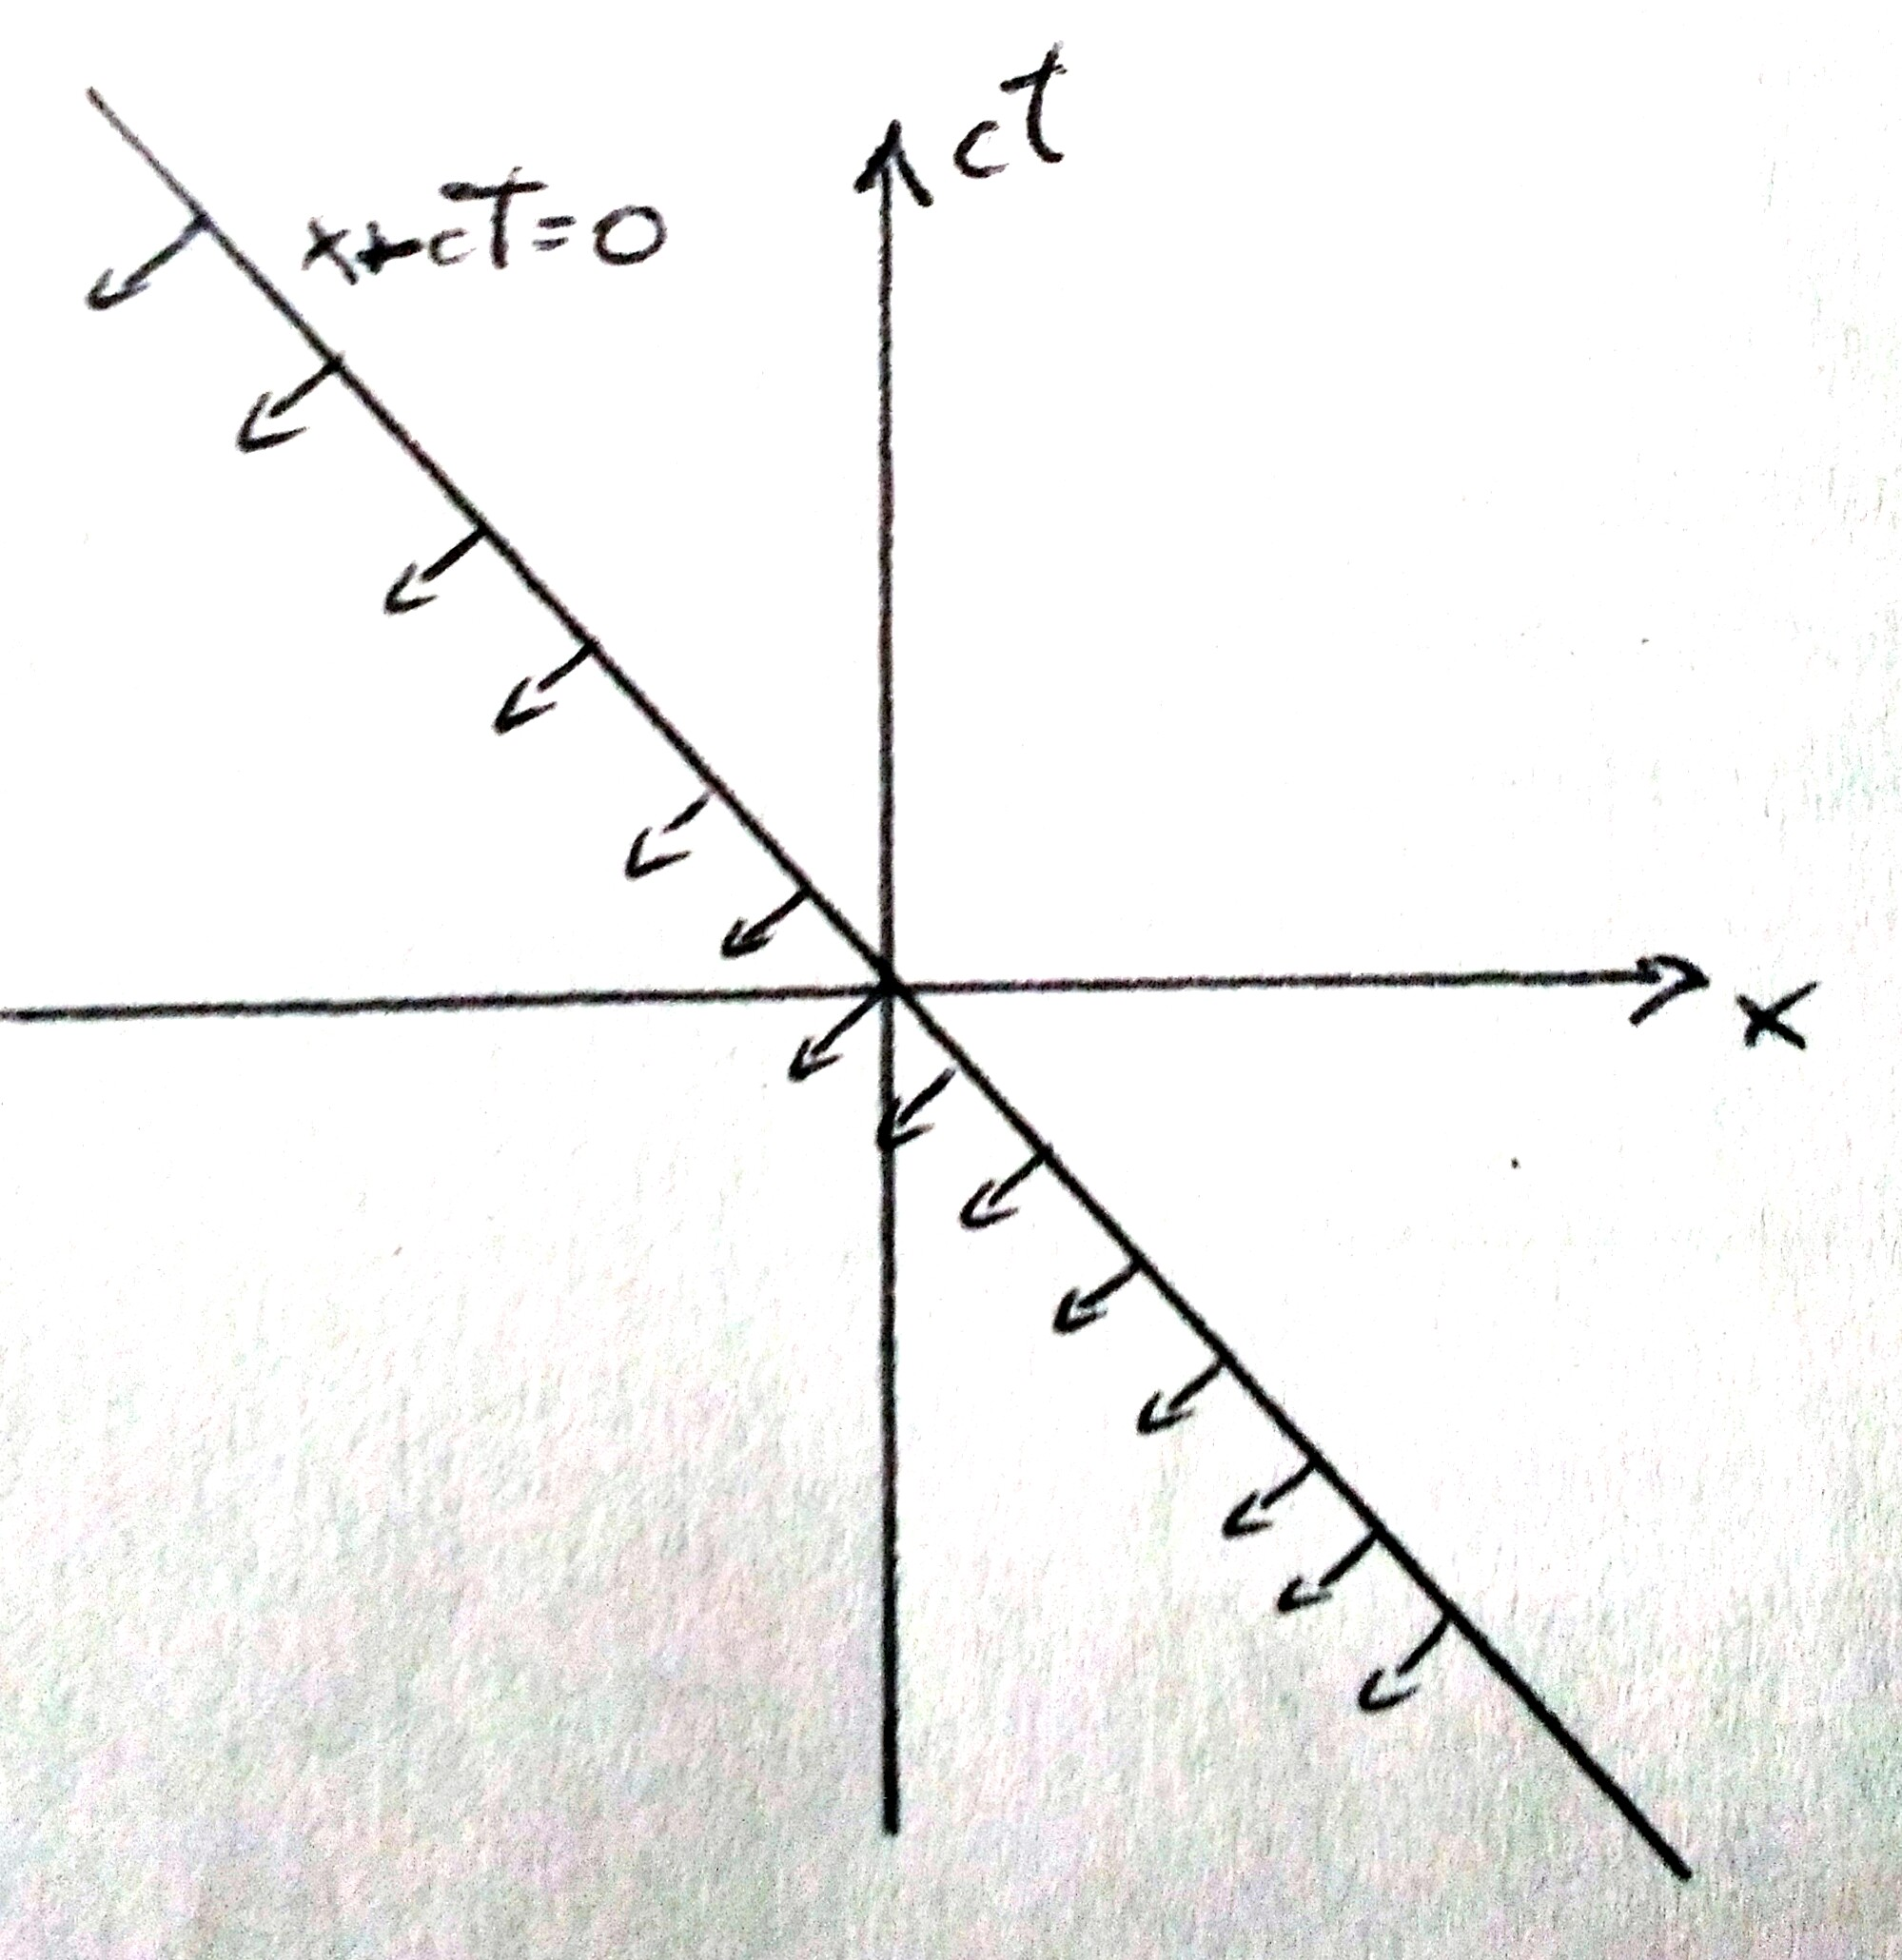
\includegraphics[width=0.3\textwidth]{images/foglio1_xt}
	\caption*{campo nel piano (x,ct): supporto su x+ct=0, direzione lungo x-ct=0}
 \label{figure:campoxt}
\end{figure}
\begin{figure}[htbp]
 \centering
 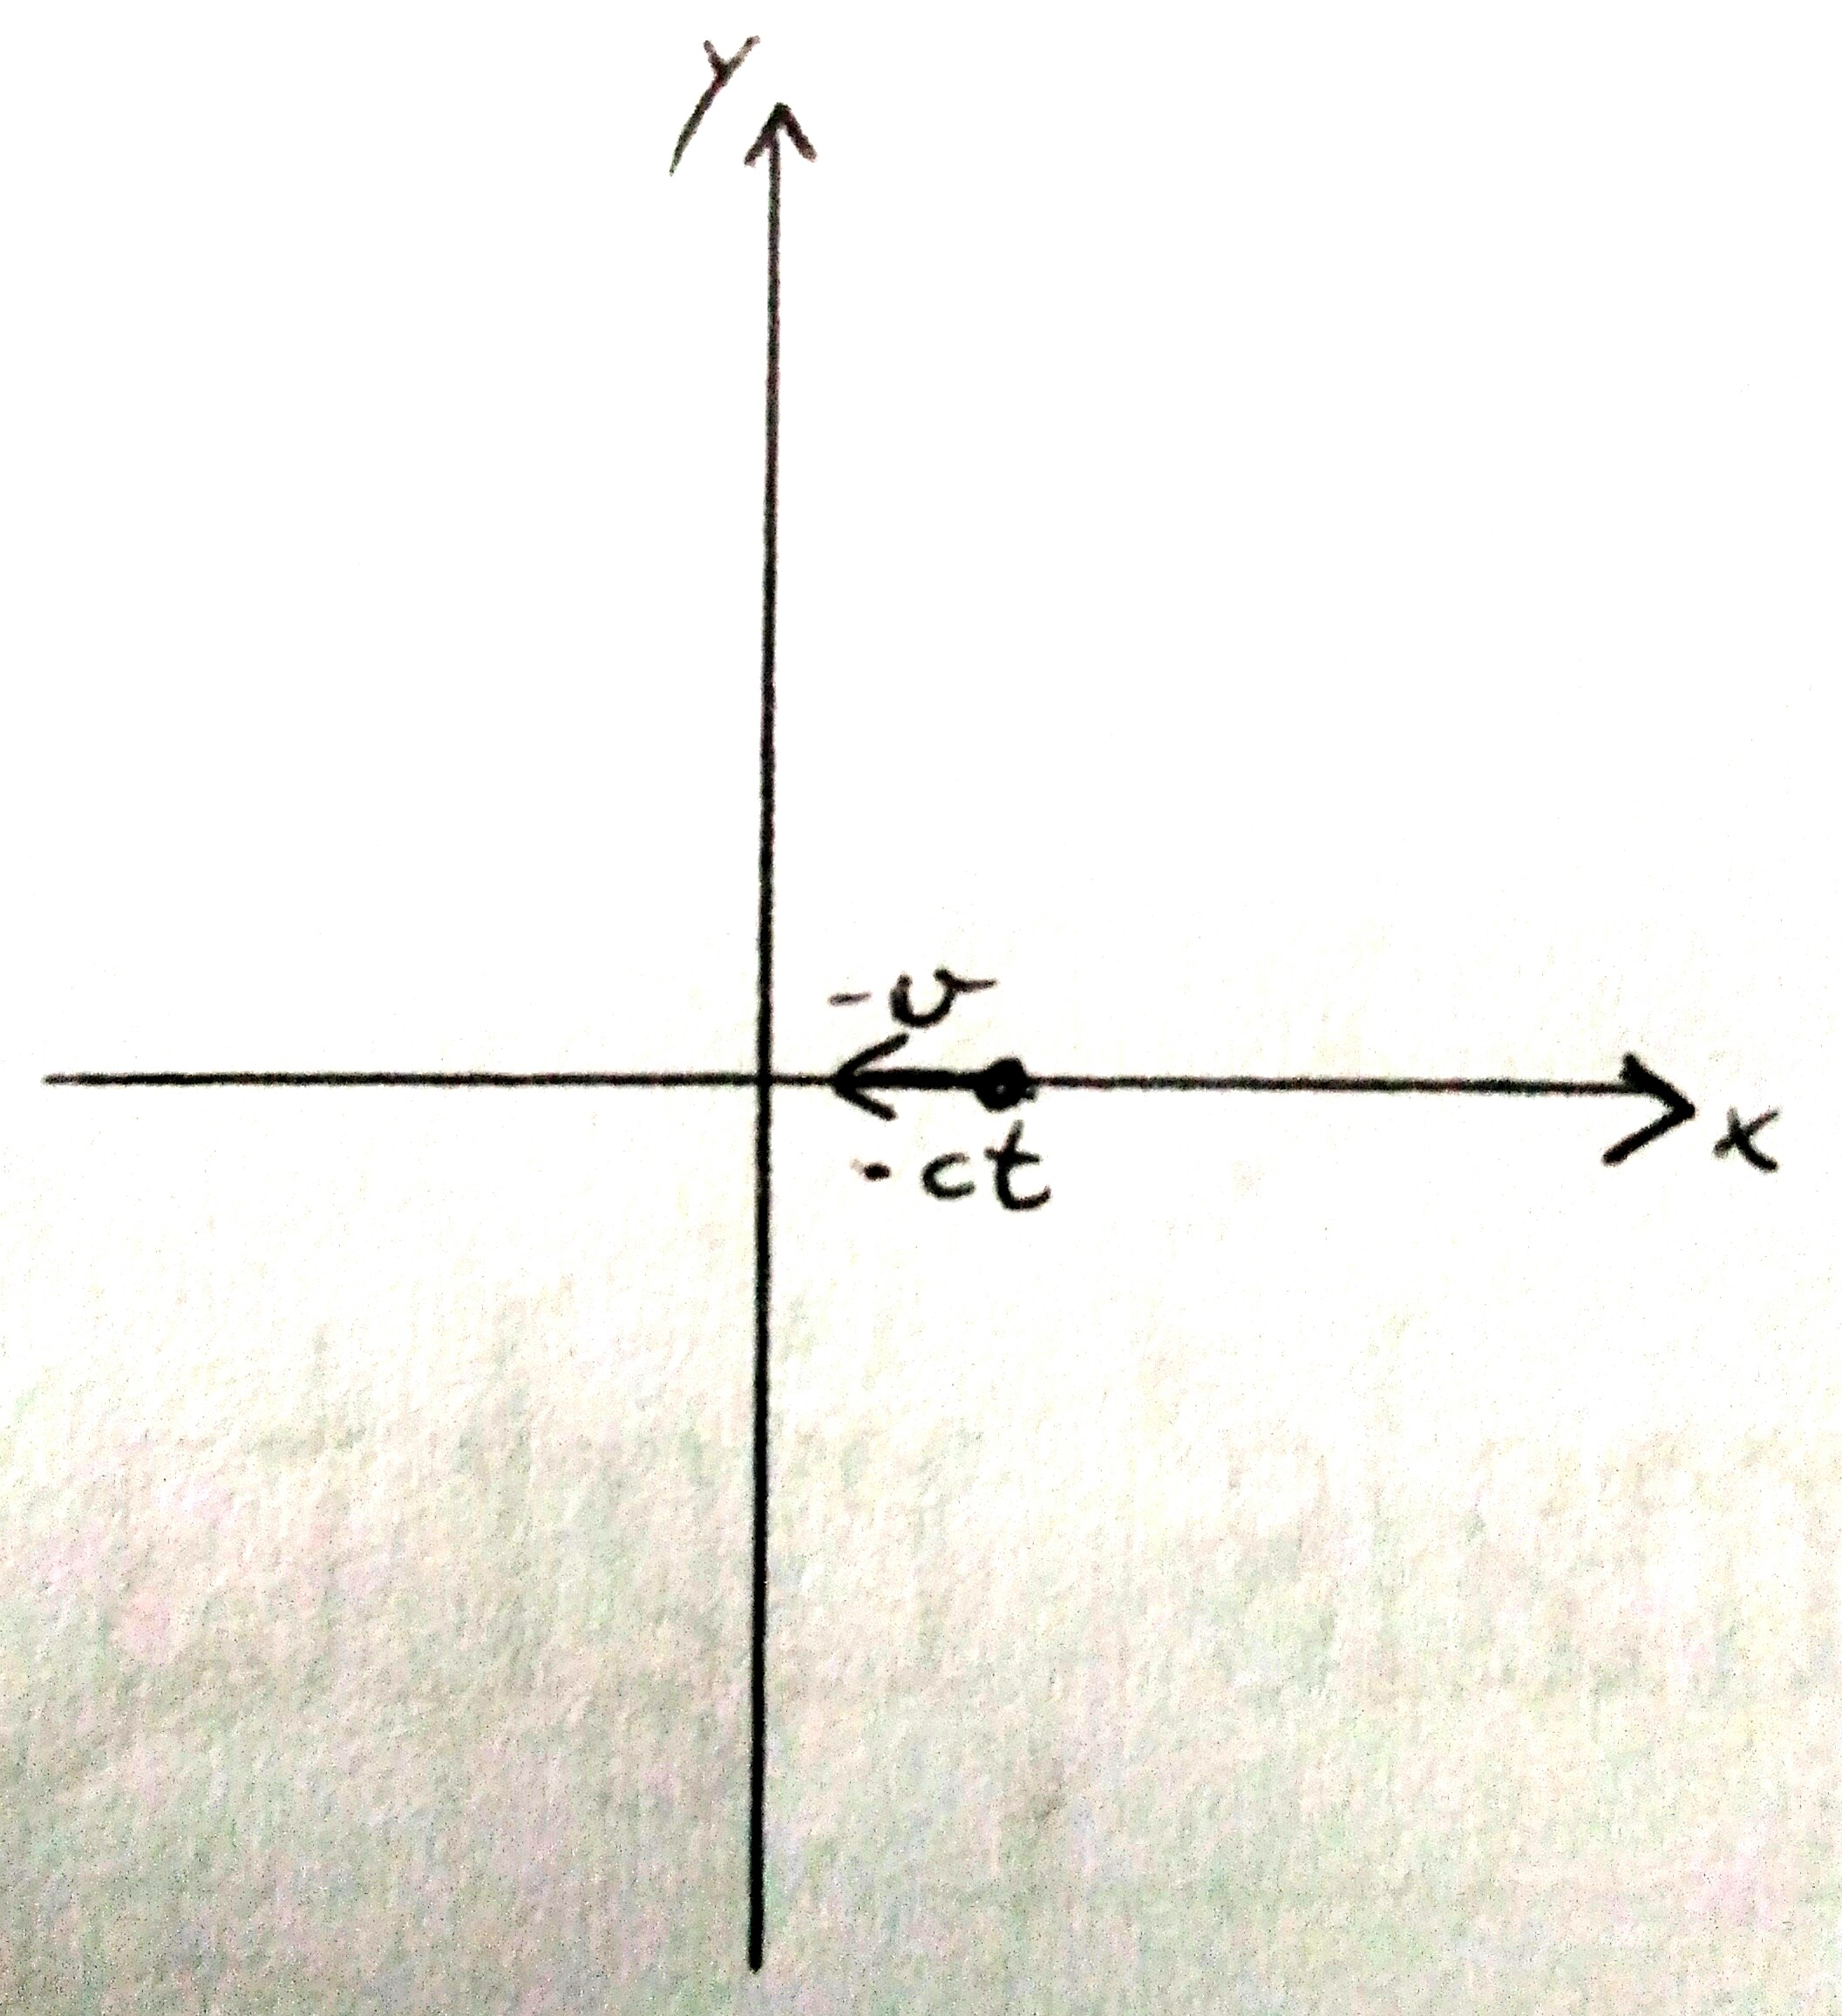
\includegraphics[width=.3\textwidth]{images/foglio1_xy}
	\caption*{campo nel piano (x,y): supporto su x+ct=0, nel punto in cui \`e la particella, diretto come la velocit\`a della particella}
 \label{figure:campoxy}
\end{figure}


 



































